\newpage
\section{Hotspot Analysis}
Heat conduction (or heat diffusion) is the process by which thermal energy spreads within a material due to temperature differences. In two dimensions, this phenomenon can be represented as heat spreading across a plate or surface over time. Numerical simulations of heat conduction are widely used in engineering, physics, and high-performance computing to predict temperature distribution and analyze thermal effects.

\begin{center}
    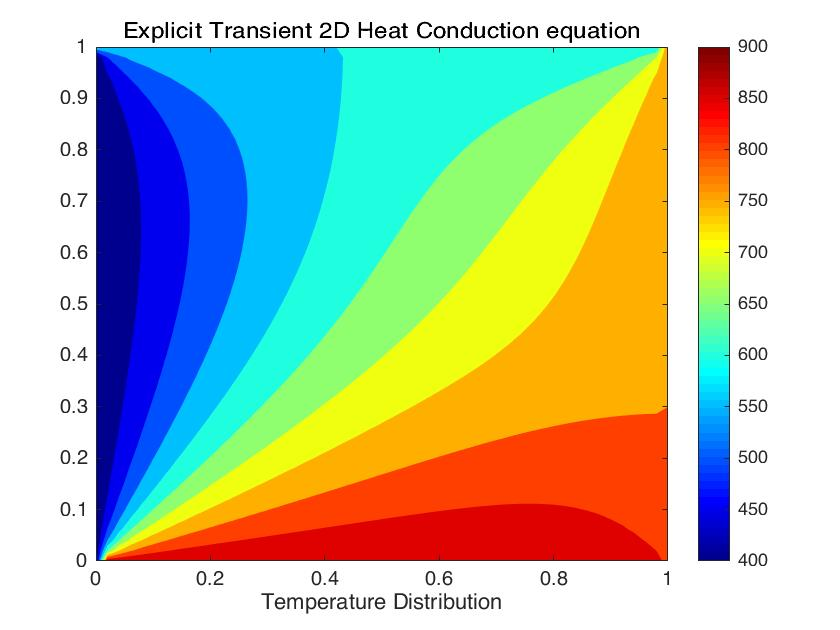
\includegraphics[width=0.6\textwidth]{assets/hotspots/heat_diffusion_simulation.jpg}
    \captionof{figure}{Illustration of 2D heat conduction simulation.}
\end{center}

\noindent
The formula to represent 2D heat conduction is given as follows:

\begin{equation}
\frac{\partial T}{\partial t} = \alpha \left( \frac{\partial^2 T}{\partial x^2} + \frac{\partial^2 T}{\partial y^2} \right)
\end{equation}

where:
\begin{itemize}
    \item $T$ is temperature;
    \item $t$ is time;
    \item $\alpha$ is the thermal diffusivity;
    \item $(x,y)$ are points in a grid.
\end{itemize}

\noindent
To solve this problem numerically, one possible finite difference approximation is:

\begin{equation}
    \label{eq:approximation}
\frac{\Delta T}{\Delta t} =
\frac{T_{i,j}^{n+1} - T_{i,j}^n}{\Delta t} = \alpha \left( 
\frac{T_{i+1,j}^n - 2T_{i,j}^n + T_{i-1,j}^n}{(\Delta x)^2} + 
\frac{T_{i,j+1}^n - 2T_{i,j}^n + T_{i,j-1}^n}{(\Delta y)^2} 
\right)
\end{equation}

where:
\begin{itemize}
    \item $\Delta t$ is the timestep;
    \item $i,j$ are indices in the grid;
    \item $n$ indicates the current timestep, so $T_{i,j}^n$ is the temperature at point $(i,j)$ at time $t=n \Delta t$, and $T_{i,j}^{n+1}$ is the temperature at the next timestep $t=(n+1) \Delta t$.
\end{itemize}

\subsection{Code Description}
This program simulates the diffusion of heat on a two-dimensional plate using the finite difference method. It includes two main implementations:
\begin{enumerate}
    \item \textbf{Reference CPU version} - \texttt{step\_kernel\_ref()} - serial implementation
    \item \textbf{Modified version} - \texttt{step\_kernel\_mod()} - intended for CUDA acceleration
\end{enumerate}

Both implementations are designed to produce the same results.

\subsubsection*{Data Layout}
The simulation uses a grid of size \texttt{ni × nj} (columns × rows).

\noindent
Temperature values are stored in a \textbf{1D array}. A macro is used to convert 2D indices to linear index:

\begin{lstlisting}
#define I2D(num, c, r) ((r)*(num)+(c))
\end{lstlisting}

\subsubsection*{Initialization}
In the beginning, the boundary points of the grid are assigned with initial \textit{random} temperatures, while the inner points update their temperature iteratively according to the formula above.\\

\begin{lstlisting}
  for (int i = 0; i < ni * nj; ++i) {
      t1_ref[i] = t2_ref[i] =
      t1[i]     = t2[i]     =
          (float)rand() / (float)(RAND_MAX / 100.0f);
  }
\end{lstlisting}

\subsubsection*{Realistic System Inizialization}

In addition to the synthetic configurations used, I also decided to simulate a more realistic scenario in order to visually inspect the physical behavior of the system.  
Specifically, I initialized the domain by placing a high–temperature square region at the center of the grid, representing a localized heat source. All remaining points were initialized with a low random temperature, mimicking environmental thermal noise.  
The initialization code is reported below:

\begin{lstlisting}
// Hot square parameters
int hot_size = 40;    // side length of the hot square
int hot_temp = 80;    // temperature of the hot region
int hot_i0 = ni/2 - hot_size/2;    // center coordinate in i
int hot_j0 = nj/2 - hot_size/2;    // center coordinate in j

for(int j = 0; j < nj; j++){
  for(int i = 0; i < ni; i++){
    int idx = I2D(ni, i, j);
    
    if(i >= hot_i0 && i < hot_i0 + hot_size && 
        j >= hot_j0 && j < hot_j0 + hot_size)
    {
      // heat source
      temp1[idx] = temp2[idx] = (float)hot_temp;
    }
    else
    {
      // random background
      temp1[idx] = temp2[idx] = (float)rand()/RAND_MAX*30.0f;
    }
  }
}
\end{lstlisting}

\noindent
The source code can be found in \texttt{src/image.cu} and the script used for the visualization was done with Matlab (more details in: \texttt{src/realistic\_simulation.m})\\

\noindent
The visual outcome of this configuration is discussed in Subsection~\ref{subsec:realistic_system_simulation}.


\newpage

\subsubsection*{Execution}
The core of the simulation is inside the \texttt{step\_kernel()} function, which implements the approximation described in formula \eqref{eq:approximation}, shown below.

\begin{lstlisting}
void step_kernel_mod(int ni, int nj, float fact, float* temp_in, float* temp_out)
{
  int i00, im10, ip10, i0m1, i0p1;
  float d2tdx2, d2tdy2;

  // loop over all points in domain (except boundary)
  for ( int j=1; j < nj-1; j++ ) {
    for ( int i=1; i < ni-1; i++ ) {
      // find indices into linear memory
      // for central point and neighbours
      i00 = I2D(ni, i, j);
      im10 = I2D(ni, i-1, j);
      ip10 = I2D(ni, i+1, j);
      i0m1 = I2D(ni, i, j-1);
      i0p1 = I2D(ni, i, j+1);

      // evaluate derivatives
      d2tdx2 = temp_in[im10]-2*temp_in[i00]+temp_in[ip10];
      d2tdy2 = temp_in[i0m1]-2*temp_in[i00]+temp_in[i0p1];

      // update temperatures
      temp_out[i00] = temp_in[i00]+fact*(d2tdx2 + d2tdy2);
    }
  }
}
\end{lstlisting}
\paragraph*{Note:} The formula corresponds \eqref{eq:approximation} to lines 18–23 in the above code.

\subsubsection*{Verification}
After all timesteps, \texttt{temp1\_ref} holds the CPU reference results, while \texttt{temp1} holds the modified version results. If the error exceed a threeshold (e.g. 0.0005), the simulation is considered correct.

\begin{lstlisting}
  float maxError = 0;

  for( int i = 0; i < ni*nj; ++i ) {
    if (abs(temp1[i]-temp1_ref[i]) > maxError) { maxError = abs(temp1[i]-temp1_ref[i]); }
  }

  // Check and see if our maxError is greater than an error bound
  if (maxError > 0.0005f)
    printf("The error is NOT within acceptable bounds.");
  else
    printf("The error is within acceptable bounds");
\end{lstlisting}

\subsection{Project Structure}
The \texttt{homework2} project is organized into four main directories:
\begin{itemize}
    \item \textbf{build}: contains the compiled executables.
    \item \textbf{reports}: stores the reports generated with the \texttt{-qopt-report} flag.
    \item \textbf{src}: includes the source code files.
    \item \textbf{metrics}: scripts that run the executables in \texttt{build} and save performance metrics.
\end{itemize}

\subsection{Profiling}
For performance profiling, I chose to use the university workstation, using Intel's profiling tools: \textbf{VTune} and \textbf{Advisor}. The code was compiled using the Intel Compiler (\textbf{ICX}) with the following flags: \texttt{-O3 -g -xHost} to enable high optimization, generate debug information, and target the host CPU architecture.

\subsubsection*{Simulation Parameters}
The analysis was conducted considering data size resulting in a sequential execution time of $\sim 30$ seconds, by setting:

\begin{itemize}
    \item $nstep = 200$
    \item $ni = 20'000$
    \item $nj = 20'000$
    \item $size = ni \times nj = 400'000'000$
\end{itemize}

\subsubsection*{Compiler Reports}
In addition to runtime profiling, I also examined the compiler optimization reports generated with the flag \texttt{-qopt-report}. These reports provide insights on which loops and functions the compiler was able to optimize or vectorize.

\subsubsection*{Advisor Roofline Analysis}

\begin{figure}[H]
    \centering
    \includegraphics[width=0.8\textwidth]{assets/advisor/seq\_roofline.png}
    \caption{Roofline analysis of the sequential baseline code.}
\end{figure}

\begin{figure}[H]
    \centering
    \includegraphics[width=0.8\textwidth]{assets/advisor/seq\_survey.png}
    \caption{Advisor Survey.}
\end{figure}